\documentclass[twocolumn]{article}
\usepackage{amsmath}
\usepackage{hyperref}
\usepackage{usenix} 
\usepackage{graphicx,float}
\begin{document}

\title{Anomaly Detection on Floodlight}
\author{Irtiza Ahmed Akhter \\ 
		\texttt{irtiza@cs.wisc.edu} 
		\and Aditya Prakash\\
		\texttt{aprakash6@wisc.edu}}

\maketitle

\abstract
Efficient traffic analysis in an IP network has been an interesting area of study. The existing Internet hosts a diverse set of applications. In that any application can generate any type of traffic destined to anyone. In this chaotic setup it is practically impossible for the network administrator to extract important traffic pattern. Traffic monitoring has its own salient incentives including anomaly detection, find resource consumption or simply troubleshooting. Prior works in this area lack are unidimensional and produce excessive detail in the report. \emph{Autofocus}\cite{estan} is an offline traffic analyzer that addresses the challenges to generate multidimensional and compact report of an IP network.  In this work we propose a design to solve a similar problem in software define networks (SDN). We implemented a prototype of this design on top of \emph{Floodlight} \cite{floodlight}. This module essentially solves a traffic characterization problem leveraging the floodlight controller to perform an online analysis of live traffic compared to the offline approach of \emph{Autofocus}. In addition to that this prototype also provides a simple framework that exploits this traffic clustering solution for anomaly detection based on signatures. 



\section{Introduction}

Internet today consists of various kinds of traffic generating from streaming media, content delivery networks, peer-to-peer applications and also from anomalous applications. The Internet model encourages the notion of flexibility. The same philosophy caused it to be exposed to this diverse set of applications. Consequently Internet has become open target for different types of attacks including denial of services, network worms, distribution of bot net code, etc. Network management and administration practically have become a nightmare for the network personnel. As a result thus far quite a number of works have been proposed and reported in the literature that focus on automating this tedious process in a traditional IP network. This area of research is known as the traffic characterization problem and the goal here is to identify interesting traffic patterns in the network, mostly to troubleshoot and to detect anomalous behaviors efficiently.  Almost all of the works translate this problem to one of the popular clustering problems. These methods usually take raw traffic flows as input and perform an offline analysis. Although unlike the online approach offline method has the luxury of leveraging more computational resources, it has its own problems. Firstly regardless of the exact mechanism used to solve the clustering problem the analyzer will have to extract sufficient dimensions from the input in order to expose interesting problems. At the same time it must be careful in report generation to remove any unnecessary and uninteresting traffic clusters. These two goals are conflicting and in a traditional IP network these imply to adopt a very expensive algorithmic approach to process a large chunk of raw traffics. Software defined networks (SDN) has made things easier, but it does not omit the incentives for traffic monitoring. As a matter of fact traffic analysis on SDN needs to be done online and it imposes a different set of challenges on the design in addition to the requirements of generating reports with sufficient dimensionality and with meaningful clusters only. First of all, the overall design needs to be fast, efficient and lightweight so that it does not introduce significant computational overheads and must not interfere with the ongoing traffic. Next the design will have to be robust and scalable so that a single detector can monitor a large network and cope with the flood of live traffic. And finally it must produce accurate report for any given network. In other words, it must be able to capture the traffic patterns accurately and deal with the overlapping patterns without any error probability. In this work we present a design of a detection mechanism that works on SDN and achieves the aforementioned goals. This design implements the basic idea of traffic clustering using multiple dimension presented in \cite{autofocus} and presents its own solution to characterize online traffic on SDN. We then implement a prototype of this design as module in Floodlight   \cite{floodlight} for evaluating the design and to provide directions to future researches. \\\\
The remainder of this report is organized as follows. In Section~\ref{sec:relatedwork} we briefly discuss a number of related works in this  area followed by a more thorough discussion on Autofocus in Section~\ref{sec:autofocus}. We then move on to describing the design and implementation of our solution in Floodlight for traffic characterization in Section~\ref{sec:adonfloodlight}. In Section~\ref{sec:evaluation} we present our evaluation plans and some results from the prototype we developed. Next we thoroughly discuss a list of future works in Section~\ref{sec:futurework} to improve the current implementation. We also present our initial suggestions to address each of the enhancements in the same section. In Section~\ref{sec:summary} we summarize this work and point out the highlights. 


\section{Related Work}
\label{sec:relatedwork}
The majority of existing network anomaly detectors are based on a standard set of pre-defined patterns to identify well known aspects of network traffic. Any traffic flow that does not fall under these patterns are considered anomalous in this model. 
Also the canonical model for anomaly detection usually works on one or two fields of the IP header to isolate flows into clusters. In contrast to that mode \emph{Autofocus}, a more recent work used five fields of the IP header to provide sufficient dimensionality in the report.  Most of the existing techniques use a flow profiling technique. Cisco’s \emph{NetFlow Analyzer} provides a detailed record of the traffic observed on the network. It keeps track of packets and categorizes them based on IP flows. It uses 7 fields instead of the standard five including the \emph{type of service} and \emph{input sub-interface}. This approach provides excessive detail and cannot be used to group several flows into many different clusters.  \emph{FlowScan} also falls under this category of network analyzers. It uses Cisco routers to send flow-export UDP packets to a host running a specialized application that further analyzes the flows. Obviously for a large network this method causes large computational and network overheads. \emph{FlowMatrix} \cite{flowmatrix}  is also another approach that uses \emph{NetFlow} records from Cisco routers and builds a detailed multidimensional behavioral model of the network. Later, it compares the measured parameters with the models and detects abnormalities. A major problem with all the above approaches is that they can only be used on Cisco routers and thus are proprietary. There are several approaches that are signature based as opposed to anomaly based. \emph{Snort} \cite{snort} and \emph{Bro} \cite{bro} examine traffic for known attacks using predefined rules specified by security experts. The major advantage of our approach is that it adopts a combination of signature based and anomaly based detection. Especially with the widespread growth of SDN, it is necessary to leverage the features of SDN to construct an online detection tool. Our work is primarily built using the idea of \emph{Autofocus} \cite{autofocus} and therefore we present the mechanics of Autofocus throughly in the next section. While doing that we also highlight the high level design differences between Autofocus and our solution.

\section{Dissection of Autofocus}
\label{sec:autofocus}
Autofocus \cite{autofocus} is a traffic analysis tool for IP networks that can perform offline analysis. It focuses on dynamically defined traffic clusters instead of individual flows or other predefined aggregates. Autofocus was developed to meet three key practical requirements, namely dimensionality, level of detail and utility. Dimensionality represents the accuracy of the generated report. For example traffic report classified on a single attribute is not going to be very helpful for the network administrators and essentially will hide many interesting and important behaviors. On the contrary, too many dimensions are likely to cause infeasible amount computational overhead as Autofocus works on large trace of flows at a time. So the dimensionality requirement constraints the Autofocus design to find a middle ground between these two sides. Working on more than one dimension will likely produce some uninteresting clusters if done in the naive way. In a practical scenario the situation is worse for five dimensions. As a result the naive report will contain excessive uninteresting detail about the clusters compared to the meaningful ones. Note that it is the network administrator\rq{}s time Autofocus aims to to optimize, not any other resource and producing such excessive detail in the report simply does not help the goal. Therefore it adopts the second requirement that filters out those uninteresting traffic clusters for the network administrator. The final requirement assures that Autofocus\rq{}s design stays within the well understood IP header to allow the network administrator to take necessary actions on specific occasions; a random combination of bit patterns in the payload  would not help the administrator at all in doing that. In the following sections we will see the different parts of the design as well as discuss the components of the implementation.

\subsection{Design of Autofocus}
Autofocus uses the same five tuple our solution uses to address the \emph{insufficient dimensionality} problem. The fields are source IP, destination IP, protocol, source transport port and destination transport port. Its multi-dimensional report generation works on top separate unidimensional reports. But from a high level the tool has three major components. A traffic parser that parses raw network flows only with IP headers. A cluster miner that implements the \emph{compute} and \emph{compress} operations described in the following section to generate the final report. The same component also implements the delta generation algorithm. And finally a visual display that does some post processing for better usability. These post processing include mapping raw field information (e.g. IP address) to real world objects (ISP name), categorizing traffic based on the input provided by the administrator, etc. We will elaborate further on the specific actions in the following section.

\subsection{Workflow of Autofocus}
Autofocus provides four separate operations to maximize the effectiveness of a traffic report. In this section in order to understand the workflow of Autofocus we briefly go over those operations. For space limitation we omit the unnecessary low level details and we refer the more interested readers to \cite{autofocus} for complete description. 

\begin{enumerate}
\item \textbf{Compute: } This operation computes and extracts the identity of all \emph{interesting} clusters from a raw trace of traffic. This filtering is done based on a predefined threshold for resource consumption. For a single dimension the compute operation uses a brute-force techniques to generate this initial identities. This works well for a set with only small number of members, for example the \emph{protocol} field in the IP header can only have one of three values (UDP / TCP / ICMP). However for other fields like IP addresses this is not feasible and what Autofocus does instead is that it creates a tree following the natural IP hierarchy out of the raw trace. \footnote{The tree contains the unique IP addresses as leaves and different subnets as internal nodes.} Then the compute operation traverses the tree in  post order twice. In the first pass it calculates the counts of each of the child nodes and in the second pass it updates the counts of the internal parent nodes by adding up the counts of the children. For the multidimensional situation with a dimension of $k$ ($k=5$ in this case), this compute operation essentially first solves $k$ unidimensional problems and then combines the clusters.

 \item \textbf{Compress: } Having found the base set of clusters the next step is to compress the set to filter out the meaningful clusters only. This operation uses a number of filtering heuristics for this task and as a result this design trades accuracy for conciseness. A sample heuristic is based on the following observation. If a cluster $C$ can be inferred by another cluster $C`$ then remove $C$ from the report. This causes unnecessary complication in determining the inference relationship. However the natural IP hierarchy can be leveraged to get this task done more efficiently. This step then again traverses the filtered tree in post order to eliminate the clusters based on their counts. This method however uses an estimation of counts and thus is subject to an error probability. 
 
\item \textbf{Compute Deltas: } This goal of this task is to generate a report to indicate which of the traffic clusters have changed since the last report and to what extent. This is an auxiliary portion of the original report and does not affect the actual compute and compress tasks anyway. Although the same two tasks make it very hard for Autofocus to compute these deltas. Because the compress operation omits any cluster below the usage threshold. So the presence of a cluster in a past report does not assure the presence of the same in any of the future reports and vice versa. In addition to that one can debate to compute the relative changes opposed to the absolute changes to make the task easier. However Autofocus uses heuristics based on observations to measure absolute changes.  

\item \textbf{Prioritize: } This operation is responsible for organizing the final clusters in the traffic report based on some weight. Autofocus calculates \emph{unexpectedness} as the weight for each cluster. Unexpectedness indicates how far a cluster (or a flow) is deviated from the uniform or expected behavior in terms of contribution. A number close to $100\%$ indicates the ideal and uniform situation and  any value greater or less than $100\%$ makes the cluster interesting to the administrator. 

\end{enumerate}

		
\subsection{Discussion}
In this section we offer a discussion on the different ways out solution differs from that of Autofocus and the pros and cons of the same. First of all, we failed to convince ourselves about the claim made in \cite{autofocus} that it can automatically classify new traffic patterns \emph{without a priori} information on the traffic structure. On the contrary to this claim according to the description of the implementation the tool does define clusters based on a preliminary raw analysis of the given trace. So we believe that Autofocus needs a priori information like traffic patterns or signatures to perform the analysis. The case study of SD-NAP also corroborates our claim. In that Autofocus was trying to detect the \emph{Sapphire} worm. Initially Autofocus produced the spike based on resource consumption in the \emph{other} category. That led the administrator(s) to drill down further and filter traffic by port numbers to find out the infected port , $1434$ which then in turn was used to generate further analyses to detect the warm. Our solution of anomaly detection and traffic characterization can do the same only in an online manner and with much less overhead and re-computations \footnote{Assuming the worm is still in action in our case upon noticing the spike an administrator could easily add filtering rules including port specific rules without shutting down anything.}. Moreover cluster extraction from enormous chunk of raw traffic is unnecessary in our case as the system feeds the detection module real time traffic data as they are observed by the network. And finally the compute operation in Autofocus makes several passes to solve the unidimensional problems followed by an algorithm to combine the dimensions. Unlike that our solution initiates the detection module with clusters with multiple dimensions. It incrementally builds the solution as traffic flows are detected without interfering with the traffic of course. This way our solution avoids all the expensive and time consuming computation to generate a multidimensional report.  Autofocus compresses the report based on simple filtering heuristics and estimates the count in the traffic. On the contrary our solution does not use any heuristic and does not use the notion of estimated counts. Instead it leverages Floodlight and the SDN architecture to measure the actual counts. We like the idea of computing deltas of traffic clusters between two monitoring intervals. We initially planned to include the support for this in the data structures of our solution, but decided to mark this as a future work due to time constraint. However unlike Autofocus computing deltas in our solution should be straight forward. Because no information is ever lost from the controller\rq{}s perspective. It is only hiding the unnecessary ones from the report. Therefore deltas can be computed more efficiently in our design. Prioritizing traffic clusters based unexpectedness is another feature our solution lacks. Although we think unexpectedness assigns weight to clusters meaningfully, we believe using uniform behavior in today\rq{}s real world traffic might cause to raise some false alarms. In any case further study should be done before including any cluster prioritization mechanism in our solution.


\section{Anomaly Detection On Floodlight}
\label{sec:adonfloodlight}
As we mentioned earlier that our goal is two fold. We want to come up with a design of module for Floodlight that will perform an online analysis not only to detect anomalies based on signatures but also to generate real time traffic report for the network administrator. This desired solution should have both sufficient dimensionality and must omit any uninteresting clusters. For multiple dimensions we too use the five tuple (source IP, destination IP, source transport port, destination transport port, network protocol) to define a signature. In order to achieve that we propose two different approaches to work with Floodlight. For both of these approaches we install flow rules at the switch to match a desired signature. For future reference we call these approaches \emph{aggressive approach} and \emph{laid back approach} respectively. Both aggressive and laid back approaches require a priori information about traffic patterns to filter out traffic clusters as well as to bootstrap the anomaly detection module. However the gains of the latter approach are significantly large compared to the former one. Therefore in this work we implemented a prototype module using the laid back approach. In the next two sections we discuss these design approaches from a high level. We also describe the challenges associated with each of the approaches and our reasoning for choosing one over the other. Without the loss of generality the following discussion in this section assumes there is only one switch in the network. 

\subsection{Aggressive Approach}
The first approach is called \emph{Aggressive Approach} or a top down approach and works as follows. We initiate the detector with some simple base signatures. For example, a signature like (*,*,*,*,*) at every switch will capture all the flows. However, in order to make detection more efficient we should initiate the detection unit with more than just one cluster. Once these signatures are installed the switch starts counting the number of packets and the number of bytes transferred for each flow. The detection unit on floodlight will only react when the size \footnote{Cluster size can be defined as packet counts or byte counts or both} of a specific cluster goes beyond the predefined \emph{clustering threshold}. Once the threshold is reached, the detection unit will react by installing more specific rules at the switch. The detection unit may decide these specific rules based on predefined logics. For the above example it may decide to start with installing rules for $/16$ subnet and keeping track of the counts for this new cluster. After repeating the last step several times eventually the detection unit will be able narrow down to a cluster responsible for using the major portion of traffic and will be able to report and/or take action against the culprit cluster to the administrator. \\\\
The first problem with this approach is that there is no way for the module to collect information for each flow. Like \emph{Autofocus} this module does not work on pre-collected raw traces. As a result of having no information it is impossible for the detection module to generate any report at all. It can only report cluster of flow(s) that consumes resources beyond a predefined threshold as a whole. Next the logic for narrowing down the detection tree to install more specific rules is not straightforward at all. It will have to apply heuristics to prune the search space and reach down to the source of a problem. Moreover instrumenting these rules frequently at the switch is not easy and will likely interfere with the existing learning switch and forwarding modules of Floodlight. As a result there is a risk of packet drops during detection. In addition to all these there is a time delay between the first detection in the top level cluster and the detection of the leaf level clusters. During this period the problematic traffic could just stop transmitting before the controller reached a point where it can extract the five tuple. For these reasons we did not implement this approach. However this method can still detect traffic patterns by having anomaly signatures as input. 


\subsection{The Laid Back Approach}
The next method that we propose and the one we have implemented in our prototype is called the \emph{Laid Back Approach}. This method can be thought of as a mix of \emph{top-down} and \emph{bottom-up}. This method starts working on the problem and builds the results incrementally as new flows come in. As a result the solution to each of the goals (anomaly detection, traffic characterization, elimination of excessive detail, lightweight robustness, etc.) becomes simpler from an algorithmic perspective. In this method the detection unit will collect statistics from both the parent and child nodes of a cluster tree (see Figure~\ref{clustertree}) including the leaves. The exact mechanism will work as follows. It will first omit any forwarding modules that Floodlight uses to route traffic. Then just like the aggressive approach it will start with a number of signatures to initiate the base clusters. Note that these signatures can represent simply interesting traffic pattern or any pattern of known anomalies. Then for every unique flow \footnote{By unique we mean a unique combination of the five fields} the detection unit will first extract the five tuple from the flow and create a cluster in the controller's memory. Then it will instruct the switch to install a flow rule for the exact match with configurable hard timeout \footnote{Setting out the timeout is just a configuration that needs to be tuned. For example there is no reason to keep a rule for infinite amount time \emph{on the switch} and also there is no reason to delete the rule just after 1 minute} for that unique combination of five tuple without causing any delay. The detection unit can access the flow rules on the switch in future uniquely by the identification numbers \footnote{We used the cookie field of \emph{OFFlowMod} to uniquely identify a flow in the switch. These ids are assigned and maintained by the detection unit}. After that the detection unit will run a matching algorithm for the newly created cluster. The matching algorithm's goal is to decide which of the base clusters can be a parent of the new cluster. This is essentially a many to many relationship between these two types of clusters (see Figure~\ref{fig:clusters}). Because, a single unique flow can fall into more than one base clusters and essentially a base cluster will capture a lot of unique flows. Once the parent cluster(s) are found for the new cluster, it will setup pointers in the new cluster's data structure to ensure fast access to the parents in future. The trick here is to also implement the basic learning switch functionality inside this detection unit. And once the mac address to port mappings are learned all the rules can be installed consistently without causing any packet drops. Note that in this method the detection unit will not install any of the base signatures. Initially those signatures were used to create the logical clusters in the controller's memory. So this way at any given point of time, the switch will have a flow rule for every unique flows it has seen so far subject to the timeout period and the detection module will have clusters for the same unique flows. From this point, the detection module will query the switch to get the packet and byte counts for each of these flows periodically. Once those counts are extracted it will carefully update the counts for each of the unique clusters as well as of their parent clusters and perform some simple calculations. At the same time it will mark each cluster for reporting based on the predefined clustering threshold. In other words it will include in the report only those clusters which have so far crossed the predefined clustering threshold. \\\\
Now let us point out the good features of this laid back approach. First this method allows the detection unit to collect information of every unique flows. This makes the meaningful report generation task very easy. Next anomaly detection is very straightforward given the signature. And this method does not any way cause any packet to drop and maintains the forwarding rules consistently. Moreover it is only a matter of implementation to have this design work with dynamic addition and deletion of traffic signatures. However there is a small catch with this design and that is it will cause the switch to install one rule per unique flow. But optimizations can be done. For example, using the configurable timeout settings for each rule it can delete the rule from the switch but retain the states of the deleted flow in the controller's memory. 
\begin{figure}[!ht]
\centering
	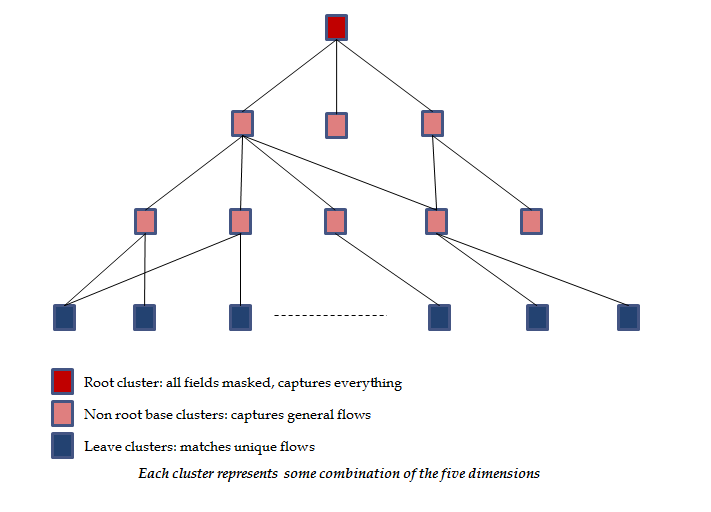
\includegraphics[scale=0.6]{images/clusters.png}
\caption{A pictorial view of the clusters created by the laid back approach}
\label{fig:clusters}
\end{figure}
\section{Implementation}
We decoupled the entire implementation of the laid back approach into five separate submodules. We describe these submodules and their functionality in this section. The five submodules are \emph{Anomaly Detector}, \emph{Detection Unit}, \emph{Cluster Manager}, \emph{Flow Manager} and \emph{Statistics Collector}. Figure~\ref{fig:design} illustrates these pieces in a parent child style tree. Statistics collection from the switch, anomaly detection and finally report generation work in separate threads. And Figure~\ref{fig:workflow} illustrates the steps of the module for a single switch.

\begin{figure}[!ht]
\centering
	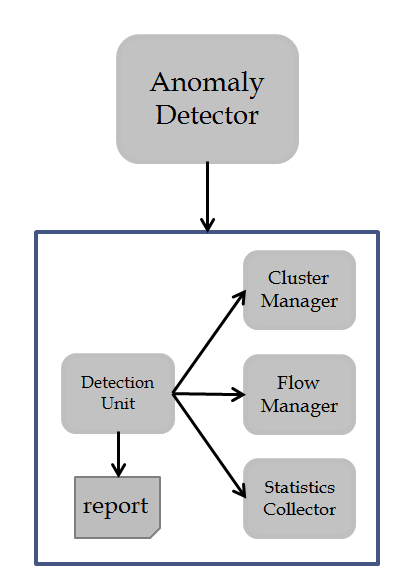
\includegraphics[scale=0.5]{images/designpieces.png}
\caption{The five pieces of the prototype. An arrow indicates a parent to child relation.}
\label{fig:design}
\end{figure}

\subsection{Anomaly Detector}
Anomaly detector is the base class and starting point for this module. It implements the necessary Floodlight listeners and maintains a per switch data structure for efficient access. Once initiated it creates an instance of the the detection unit to start the process. This same class is also responsible for cleaning up the objects for disconnected nodes. For each new flow it hands over the packet header to the detection unit for processing.

\subsection{Detection Unit}
Detection unit implements the core logics of this prototype. At first it creates a data structure to hold the traffic clusters and initiates the base clusters. As of now the base clusters need to be hard-coded in this module, but it can be easily extended to make it read from an external configuration file. It then starts the statistics collector and flow manager for each switch in the network. This module is responsible for managing all the clusters in an organized way. For every new flow it extracts the necessary fields and instructs the flow manager to create a specific flow using a unique id. At the same time it creates flow specific cluster and runs the matching algorithm. Cluster manager provides the necessary APIs to perform field specific match. Statistics collector runs in a separate thread and periodically queries the switch for new counts. Upon extracting the per flow counts detection unit then updates the counts carefully for each cluster and generates a report. During this update based on the clustering threshold it marks each cluster with a flag that is used to determine the weight of a cluster during report generation. Both report generation and statistics collection intervals are configurable via this module. 

\subsection{Cluster Manager}
Cluster manager provides a robust data structure to hold information for each cluster. These information include the fields of the five tuple namely, source IP address, destination IP address, source port, destination port and network protocol. Besides it maintains a list of pointers to  other (base) cluster(s) to establish the parent child hierarchy. Cluster manager also provides the functionality to parse a traffic signature and a flow mod into a cluster and to perform field wise matching. As mentioned earlier from a high level any traffic signature includes the five fields of IP header. Cluster manager provides us the flexibility to be as general or as specific as possible in creating these rules. In order to illustrate this further consider the example of for creating a signature with matching port numbers. With the support of the cluster manager one can add a signature with any of the following values for source (and/or destination) transport ports: a specific port number, or a range of port number (e.g. low port - high port) or none. Similarly for source and destination IP addresses one can mask any or none of the 32 bits\footnote{we only have support for IPv4 addresses currently.}. And finally this module is responsible for updating each cluster and its parents with the new counts carefully, compute the total contribution of each cluster and mark any cluster to be included during the report generation.


\subsection{Flow Manager}
Flow manager \footnote{In the actual implementation it's called \emph{Rule Maker}.} implements the interfaces to react on the \emph{packet-in} events in the controller triggered by the switch. It also includes the implementations of interacting with the switch governed by the detection unit.  This module works closely with both the detection unit and anomaly detector. These actions include composing flow mod rules from clusters, pushing packets out to the switch and install the new rules. Beside all these it includes the implementation of a learning switch and maintains a dictionary of mac address to port mappings. This map is used to install any rule consistently without hampering other flows.

\subsection{Statistics Collector}
Statistics collector is responsible for two tasks. First to query the switch for new counts for each flow and secondly to extract the necessary information from these query results in a structure that the detection unit understands. For the first task it uses Floodlight's one of the REST APIs. We use a web service that can get switch specific flows. This web service responds with a json object with all the flow entries. Statistics collector then parses these results and uses a simple data structure to store the per flow counts. As we mentioned earlier, the cookie of each flow is used as a unique id and further used by the detection unit to map each flow to a cluster.

\begin{figure}[!ht]
\centering
	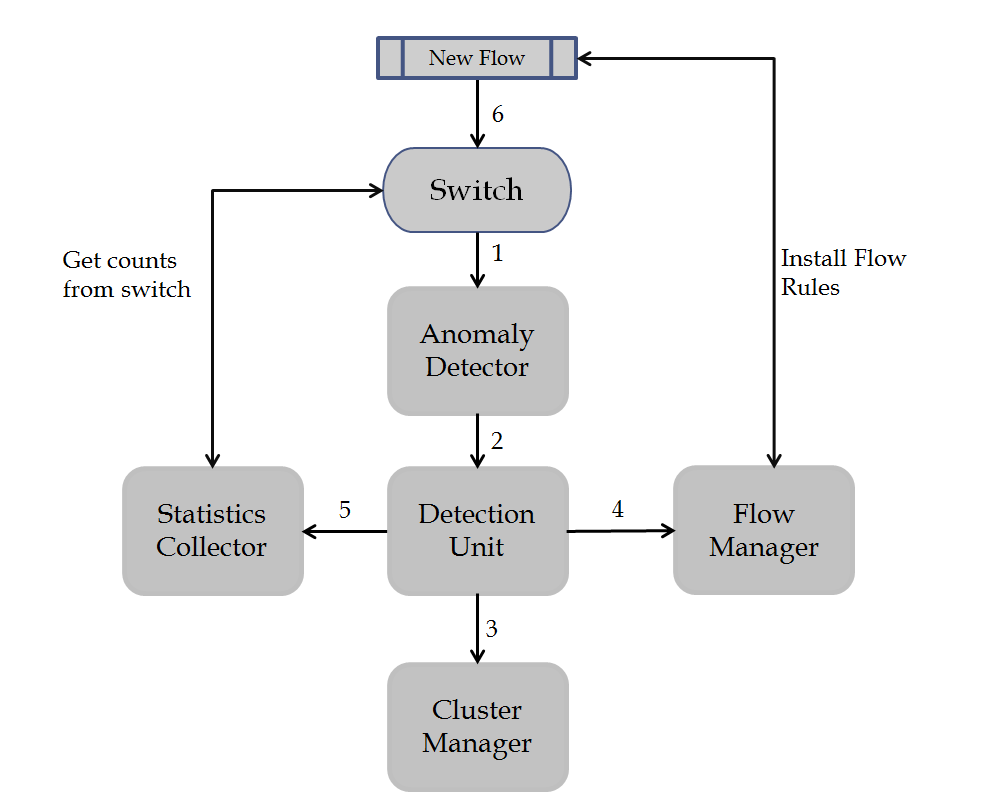
\includegraphics[scale=0.3]{images/workflow.png}
\caption{A workflow for a network with a single switch: 1) anomaly detector listens for switch connection, 2) upon detection it launches a detection unit, 3) detection unit then launches cluster manager (3), flow manager (4) and statistics collector (5) respectively, 6) once a new flow comes in, detection unit extracts the necessary fields and instructs the flow manager to install a custom rule with learning switch logic, 6.a) it then creates a cluster and runs the matching algorithm to find one or more parents for that specific flow, 6.b) statistics collector queries the switch and reports back to the detection unit with new counts and 6.c) detection unit updates the counts and generate a report subject to report generation interval}
\label{fig:workflow}
\end{figure}

\section{Evaluation}
\label{sec:evaluation}
We emphasize on four aspects of the design for evaluations, namely, accuracy in cluster generation, anomaly detection, robustness and scalability.  However note that we did not evaluate the prototype's performance in anomaly detection nor we had a chance to deploy and test the system against actual live traffic. We elaborate further on these limitations in Section~\ref{sec:futurework}.  We used synthetic traffic to evaluate the accuracy of cluster generation. We first used \emph{mininet} to setup multiple simulated network topologies with \emph{Open vSwitch}. A sample of a simple tree topology is shown in Figure~\ref{fig:simpletopology}. We tested the system with similar topologies only with variable number of hosts. We experimented with 8 hosts to 256 hosts in the mininet simulation. Next we used \emph{iperf} and \emph{ping} to generate TCP and ICMP traffic in those simulations. We also verified the results with different clustering thresholds ranging from $1\%$ to $25\%$ We wrote a number of python scripts to automate these evaluation plans in mininet while the detection module runs on Floodlight. 
\begin{figure}[!ht]
\centering
	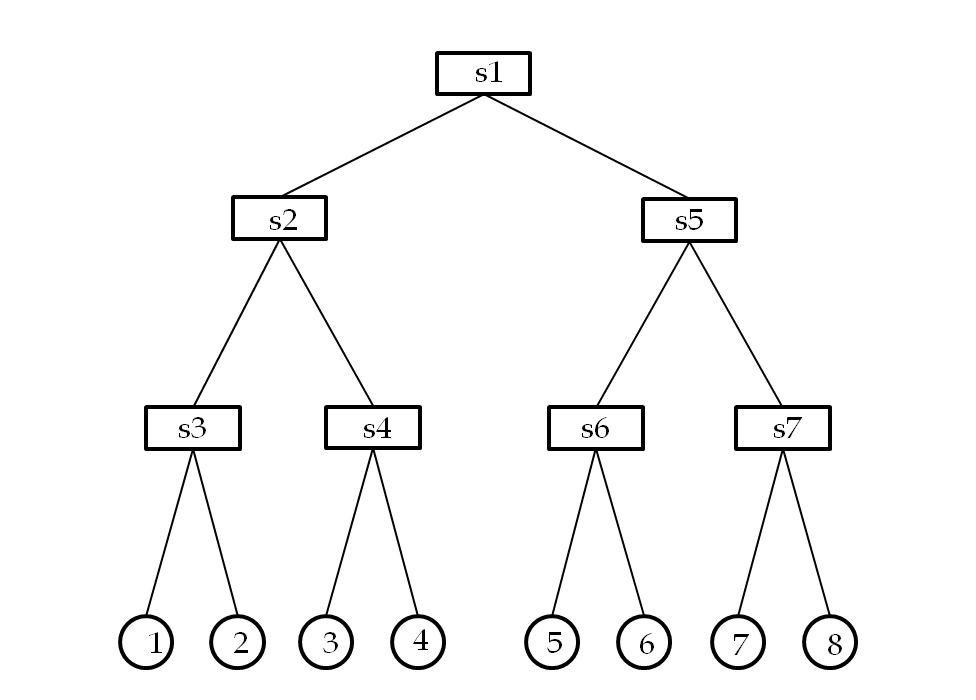
\includegraphics[scale=0.3]{images/simpleevaluationplan.png}
\caption{A tree topology on mininet with 7 Open vSwitches and 8 hosts.}
\label{fig:simpletopology}
\end{figure}

\subsection{Results}
In Figure~\ref{fig:results} we present a sample result from our experiments with 64 mininet hosts and 21 switches. For demonstration purpose this result was produced using a clustering threshold of $1\%$. We used both \emph{iperf} and \emph{ping} to simulate TCP and ICMP traffic \footnote{There were only two nodes generating the ping requests and the rest were the ICMP replies}. The anomaly detector was initialized with 7 base clusters (Cluster label 0-6) and the final report generated 15 cluster in total with 8 clusters for individual flows that crossed the clustering threshold \footnote{Floodlight port numbers are of signed short type and consequently the port numbers in the report are negatives}. As we mentioned earlier we tested the system with 256 mininet hosts to test the scalability and robustness of the controller. On a commodity laptop the controller ran and generated traffic every 1 minute without any hick-ups. 
\begin{figure*}
\centering
	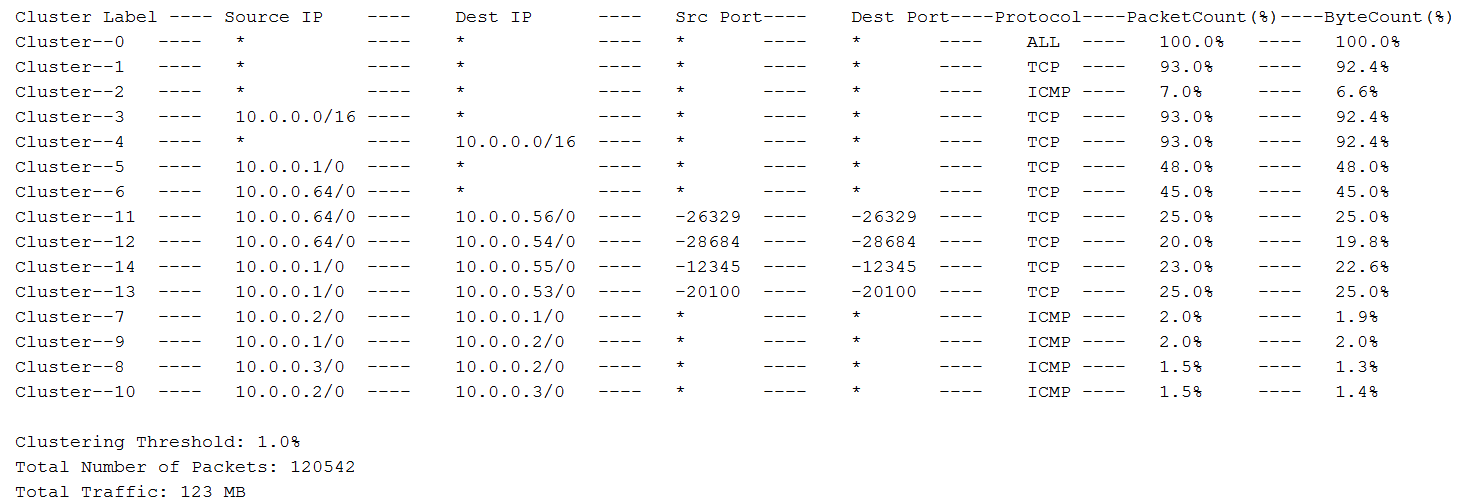
\includegraphics[width=\textwidth, height=3in]{images/results.png}
\caption{A sample report for 64 mininet hosts with clustering threshold of $1.0\%$}
\label{fig:results}
\end{figure*}



\section{Current Status \& Future Work}
\label{sec:futurework}
The current implementation successfully generates a traffic report of a network with open vSwitches. In contrast with the work of Estan et al. \cite{autofocus} currently our module does not compute the \emph{compressed report of deltas}, neither it offers any explicit prioritization based on \emph{unexpectedness}. However, our design has all the information and infrastructure to support these features. That being said, implementing these two missing pieces should not be any more than designing the algorithms and writing codes. The next thing which the current implementation does not have support for is a feature to direct traffic to a middle-ware or take appropriate action upon a detection of an anomaly. This is something we included in our initial design plans, however due to time constraint we had to omit this from the immediate to-do list. Once again implementing this feature on Floodlight is very straightforward and basically involves providing a general user friendly framework to incorporate administrative policies. This could be easily accomplished by modifying the \emph{Flow Manager} component of the current implementation. Currently our implementation does not produce any graphical analysis like \cite{estan} or \cite{flowscan}. We believe the current implementation once launched has enough information to populate interesting and meaningful real time graphs for the administrators. Therefore incorporating different network analytical model into this module would be an interesting area of future development. A user friendly graphical user interface would be another nice addition to the implementation. This tool is aimed to make a network administrator\rq{}s life easier and a simple user interface (web based or otherwise) will incentivize the early adapters. The basic functionalities of this interface should include install/uninstall traffic patterns, report and graph generation, resetting clusters, changing relevant settings, etc.  Also unlike \emph{Autofocus} this prototype does not use any mechanism to map the IP addresses and port numbers to domain names and applications respectively. An integration of a third party database of such mappings might be further useful for the end users. And lastly algorithmic optimization was not our top priority goal. Although we optimized the more obvious technicalities, a second review of the algorithms would undoubtedly be helpful to improve performance. Once optimized the software\rq{}s correctness and scalability should be throughly evaluated in an actual network with switches from different vendors against actual traffic, may be even in the presence of popular and rare anomalies. And while doing that the software should be profiled for memory and CPU usages both on switch and on the controller to quantify the required specification of the controller for a specific network.


\section{Conclusion}
\label{sec:summary}
In this project we have implemented a prototype of an anomaly detector module for Floodlight controller based on the proposed design. Our work is primarily motivated by \emph{Autofocus} \cite{autofocus}, an offline traffic analyzer for traditional IP based network. While the design of \emph{Autofocus} solely concentrated on generating multi-dimensional concise traffic reports for network administrators, our tool equally emphasizes on anomaly detection at the same time. Both of these works use the notion of \emph{traffic cluster} and solve a type of clustering problem; Only in this case the clusters are built incrementally from live traffic. According to the multiple simple evaluations reported here, the prototype successfully and correctly generated aggregated real time multi-dimensional traffic clusters. It also demonstrated impressive scalability with respect to the number of active hosts in the network. We believe with the yet to be developed features described in Section~\ref{sec:futurework} this software will be a helpful analytical tool for the SDN researchers. 

\section{Acknowledgments}
We would like to thank Aditya Akella for providing constructive feedbacks and guidance that helped us to come up with the core design of this anomaly detector on Floodlight. We would also like to thank Aditya Akella, Aaron Gember, Saul St. John and Robert Grandl for organizing the SDN bootcamp sessions. Those sessions had been tremendously helpful for us throughout the development of this project. 

\bibliographystyle{plain}
\label{references}
\bibliography{ref}

\end{document}
